\documentclass[12pt]{book}

\newcommand{\thetitle}{Think Java: How to Think Like a Computer Scientist}
\title{\thetitle}

\newcommand{\theauthors}{Allen Downey and Chris Mayfield}
\author{\theauthors}

\newcommand{\theversion}{Version 6.0 Draft -- \today}
\date{\theversion}

\usepackage{geometry}
\geometry{
    width=5.5in,
    height=8.5in,
    hmarginratio=3:2,
    vmarginratio=1:1,
    includehead=true,
    headheight=15pt
}

% paragraph spacing
\setlength{\parindent}{0pt}                      % 17.62482pt
\setlength{\parskip}{12pt plus 4pt minus 4pt}    % 0.0pt plus 1.0pt
\linespread{1.05}
\def\arraystretch{1.5}

% list spacing
\setlength{\topsep}{5pt plus 2pt minus 3pt}      % 10.0pt plus 4.0pt minus 6.0pt
\setlength{\partopsep}{-6pt plus 2pt minus 2pt}  %  3.0pt plus 2.0pt minus 2.0pt
\setlength{\itemsep}{0pt}                        %  5.0pt plus 2.5pt minus 1.0pt

% these are copied from tex/latex/base/book.cls
% all I changed is afterskip
\makeatletter
\renewcommand{\section}{\@startsection {section}{1}{\z@}%
    {-3.5ex \@plus -1ex \@minus -.2ex}%
    {0.7ex \@plus.2ex}%
    {\normalfont\Large\bfseries}}
\renewcommand\subsection{\@startsection{subsection}{2}{\z@}%
    {-3.25ex\@plus -1ex \@minus -.2ex}%
    {0.3ex \@plus .2ex}%
    {\normalfont\large\bfseries}}
\renewcommand\subsubsection{\@startsection{subsubsection}{3}{\z@}%
    {-3.25ex\@plus -1ex \@minus -.2ex}%
    {0.3ex \@plus .2ex}%
    {\normalfont\normalsize\bfseries}}
\makeatother

% table of contents vertical spacing
\usepackage{tocloft}
\setlength\cftparskip{8pt plus 4pt minus 4pt}

% The following line adds a little extra space to the column
% in which the Section numbers appear in the table of contents
\makeatletter
\renewcommand{\l@section}{\@dottedtocline{1}{1.5em}{3.0em}}
\makeatother

% customize page headers
\usepackage{fancyhdr}
\pagestyle{fancyplain}
\renewcommand{\chaptermark}[1]{\markboth{Chapter \thechapter ~~ #1}{}}
\renewcommand{\sectionmark}[1]{\markright{\thesection ~~ #1}}
\lhead[\fancyplain{}{\bfseries\thepage}]%
      {\fancyplain{}{\bfseries\rightmark}}
\rhead[\fancyplain{}{\bfseries\leftmark}]%
      {\fancyplain{}{\bfseries\thepage}}
\cfoot{}
%\rfoot{\textcolor{gray}{\tiny ThinkJava Draft \today}}

% balanced index with TOC entry
\usepackage{makeidx}
\makeindex
%\usepackage[totoc]{idxlayout}

% automatically index glossary terms
\newcommand{\term}[1]{%
\index{#1}
\item[#1:]}
% TODO: doesn't work with plastex
%\newcommand{\term}[1]{\item[#1:]}

% where to find graphics
\usepackage{graphicx}
%\graphicspath{{figs/}}

%% tweak spacing of figures and captions
%\usepackage{floatrow}
%\usepackage{caption}
%\captionsetup{
%    font=small,
%    labelformat=empty,
%    justification=centering,
%    skip=4pt
%}

% format end of chapter excercises
\usepackage{amsmath}
\usepackage{amsthm}
\newtheoremstyle{exercise}
  {12pt}        % space above
  {12pt}        % space below
  {}            % body font
  {}            % indent amount
  {\bfseries}   % head font
  {}            % punctuation
  {12pt}        % head space
  {}            % custom head
\theoremstyle{exercise}
\newtheorem{exercise}{Exercise}[chapter]

% colors for code listings and output
\usepackage{xcolor}
\definecolor{bgcolor}{HTML}{FAFAFA}
\definecolor{comment}{HTML}{007C00}
\definecolor{keyword}{HTML}{0000FF}
\definecolor{strings}{HTML}{B20000}

% syntax highlighting in code listings
\usepackage{textcomp}
\usepackage{listings}
\lstset{
    language=java,
    basicstyle=\ttfamily,
    backgroundcolor=\color{bgcolor},
    commentstyle=\color{comment},
    keywordstyle=\color{keyword},
    stringstyle=\color{strings},
    columns=fullflexible,
    keepspaces=true,
    showstringspaces=false,
    upquote=true,
    aboveskip=\parskip,
    belowskip=\parskip
}

% code listing environments
\lstnewenvironment{code}
{\minipage{\linewidth}}
{\endminipage}
\lstnewenvironment{stdout}
{\lstset{commentstyle=,keywordstyle=,stringstyle=}\minipage{\linewidth}}
{\endminipage}

% pdf hyperlinks, table of contents, and document properties
\usepackage[pdftex]{hyperref}
\hypersetup{%
  pdftitle={\thetitle},
  pdfauthor={\theauthors},
  pdfsubject={\theversion},
  pdfkeywords={},
  bookmarksopen=false,
  colorlinks=true,
  citecolor=black,
  filecolor=black,
  linkcolor=black,
  urlcolor=blue
}

% inline syntax formatting
\newcommand{\java}[1]{\lstinline{#1}} %\end{
%\newcommand{\java}[1]{\verb"#1"}
%\newcommand{\java}[1]{{\tt #1}}

\begin{document}
\setcounter{chapter}{8}


\chapter{Classes and objects}
\label{objects}

\index{String}
\index{type!String}

As we learned in the previous chapter, \java{String}s are objects.
But they are atypical in Java because:

\begin{itemize}

\item You don't have to use the \java{new} operator to create a \java{String} object.
For convenience, Java allows you to define \java{String} literals.

\item They are immutable.
You cannot edit an existing \java{String} object directly; you can only create new ones.

\end{itemize}

In this chapter, we will learn about more classes from the Java library such as \java{Point} and \java{Rectangle}.
These classes are defined in the \java{java.awt} package, so you will need to \java{import} them before running the examples.
To be clear, these points and rectangles are not graphical objects that appear on the screen.
Like strings, they contain data and provide methods for manipulating that data.
But unlike strings, you can make changes to that data directly.


\section{Point objects}

A point is two numbers (coordinates) that we treat collectively as a single object.
In mathematical notation, points are often written in parentheses with a comma separating the coordinates.
For example, $(0,0)$ indicates the origin, and $(x,y)$ indicates the point $x$ units to the right and $y$ units up from the origin.

\index{Point}
\index{class!Point}
\index{new}
\index{statement!new}

In Java, a point is represented by a \java{java.awt.Point} object.
To create a new point, you have to use the \java{new} operator:

\begin{code}
    Point blank;
    blank = new Point(3, 4);
\end{code}

\index{declaration}
\index{statement!declaration}

The first line is a conventional variable declaration: \java{blank} has type \java{Point}.
The second line invokes \java{new}, specifies the type of the new object, and provides arguments.
The arguments are the coordinates of the new point: $(3, 4)$.

\index{reference}

The result of the \java{new} operator is a {\bf reference} to the new \java{Point}.
So \java{blank} contains a reference to the newly-created object.
Here is a standard way to diagram this assignment:

\begin{center}
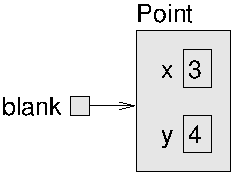
\includegraphics{figs/reference.pdf}
\end{center}

\index{attribute}

As usual, the name of the variable \java{blank} appears outside the box and its value appears inside the box.
In this case, that value is a reference, which is shown graphically with an arrow.
The arrow points to the object we're referring to, which shows the newly-created object and the two values in it.
The variables \java{x} and \java{y} are the object's {\bf attributes}.

% CSM: We already introduced memory diagrams (Ch1) and stack diagrams (Ch4).
% State diagrams are the next aspect of this general diagraming convention.

\index{state}
\index{state diagram}

Taken together, all the variables, values, and objects in a program are called the {\bf state}.
Diagrams like this that show the state of the program's objects are called {\bf state diagrams}.
As the program runs, the state changes, so you should think of a state diagram as a snapshot of a particular point in the execution.


\section{The Point class}

When you define a class in Java, you are also defining a new data type.
It is helpful to think of classes as the blueprints (or a template) for objects.
To illustrate this point (pun intended), here is a simplified version of the source code for the \java{java.awt.Point} class:

\begin{code}
public class Point {

    public int x;
    public int y;
    
    public Point(int x, int y) {
        this.x = x;
        this.y = y;
    }
    
    public String toString() {
        return "Point[x=" + x + ",y=" + y + "]";
    }
    
}
\end{code}

There are several details to note in this example.

\begin{itemize}

\item The class defines two variables (attributes) named \java{x} and \java{y} that are shared across all methods.
Because they are declared at the class level, their scope is the entire class.

\item The method \java{public Point(int x, int y)} is called a {\bf constructor}.
Its purpose is to initialize new objects, and it is called by the \java{new} operator.
Notice that it has no return type (not even \java{void}).

\item The parameters \java{x} and \java{y} in the constructor happen to have the same name as the attributes.
In order to distinguish one variable from the other, the keyword \java{this} refers to the current object.

%\item None of the variables or methods are \java{static}.
%In other words, they apply to each object of the class as opposed to the class itself.
%We will discuss this issue more deeply in the next chapter.

\end{itemize}

In practice, it's more convenient to look at high-level pictures than source code.
{\bf Unified Modeling Language} (UML) defines a standard way to visualize class designs.
Here is a {\bf class diagram} for the simplified \java{Point} class above:

\begin{center}
\vspace{1ex}
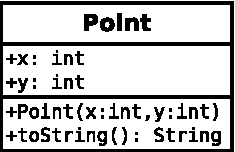
\includegraphics{figs/point.pdf}
\vspace{1ex}
\end{center}

The diagram is divided into two sections: the attributes (or variables) of the class, and the methods of the class.


\section{Instance variables}

\index{instance variable}
\index{variable!instance}

The attributes that make up an object are also called instance variables, because each object has its own copy of the variables.
Classes define new data types, and each object is an {\bf instance} of that type.

It's like the glove compartment of a car.
Each car is an instance of the type ``Car,'' and each car has its own glove compartment.
If you ask me to get something from the glove compartment of your car, you have to tell me which car is yours.

\index{dot notation}

Similarly if you want to read a value from an object, you have to specify the object you want to get it from.
Java uses dot notation for this purpose.

\begin{code}
    int x = blank.x;
\end{code}

The expression \java{blank.x} means ``go to the object \java{blank} refers to, and get the value of \java{x}.''
In this case, we assign that value to a local variable named \java{x}.
There is no conflict between the local variable named \java{x} and the instance variable named \java{x}.
The purpose of dot notation is to identify {\em which} variable you are referring to unambiguously.

You can use dot notation to build other Java expressions.
Here are several common examples:

\begin{code}
    System.out.println(blank.x + ", " + blank.y);
    int sum = blank.x * blank.x + blank.y * blank.y;
\end{code}

The first line prints {\tt 3, 4}; the second line calculates the value 25.


\section{Objects as parameters}

\index{parameter}
\index{object!as parameter}

You can pass objects as parameters in the usual way.
For example:

\begin{code}
    public static void printPoint(Point p) {
        System.out.println("(" + p.x + ", " + p.y + ")");
    }
\end{code}

This method takes a point as an argument and prints it in parentheses.
If you invoke \java{printPoint(blank)}, it prints \java{(3, 4)}.

It turns out that Java already has a way of printing \java{Point}s and other objects.
All you have to do is define a \java{toString} method, and \java{println} will call it.
For example, if you invoke \java{System.out.println(blank)} you get:

\begin{stdout}
java.awt.Point[x=3,y=4]
\end{stdout}

This format is what \java{java.awt} uses for printing objects.
It prints the name of the type, followed by the names and values of the instance variables.

As a second example, we can rewrite the \java{distance} method from Section~\ref{distance} so that it takes two \java{Point}s as parameters instead of four \java{double}s.

\begin{code}
    public static double distance(Point p1, Point p2) {
        double dx = (double) (p2.x - p1.x);
        double dy = (double) (p2.y - p1.y);
        return Math.sqrt(dx * dx + dy * dy);
    }
\end{code}

The typecasts are not really necessary; they are simply a reminder that the instance variables for \java{Point} are integers.


\section{Objects as return types}

\index{Rectangle}
\index{class!Rectangle}

\java{Rectangle}s are similar to points, except that they have four instance variables: \java{x}, \java{y}, \java{width}, and \java{height}.
This example creates a \java{Rectangle} object and makes the variable \java{box} refer to it.

\begin{code}
    Rectangle box = new Rectangle(0, 0, 100, 200);
\end{code}

This figure shows the effect of this assignment.

\begin{center}
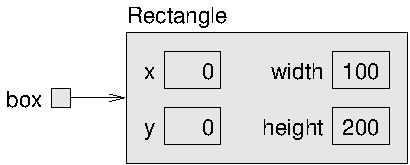
\includegraphics{figs/rectangle.pdf}
\end{center}

If you print \java{box}, you get:

\begin{stdout}
java.awt.Rectangle[x=0,y=0,width=100,height=200]
\end{stdout}

Again, this output is the result of a \java{toString} method that knows how to display \java{Rectangle} objects.

\index{return}
\index{statement!return}

You can write methods that return objects.
For example, \java{findCenter} takes a \java{Rectangle} as an argument and returns a \java{Point} that contains the coordinates of the center of the \java{Rectangle}:

\begin{code}
    public static Point findCenter(Rectangle box) {
        int x = box.x + box.width / 2;
        int y = box.y + box.height / 2;
        return new Point(x, y);
    }
\end{code}

Notice that you can use \java{new} to create a new object, and then immediately use the result as the return value.


\section{Mutable objects}

\index{mutable}
\index{object!mutable}

You can change the contents of an object by making an assignment to one of its instance variables.
For example, to ``move'' a rectangle without changing its size, you can modify the \java{x} and \java{y} values:

\begin{code}
    box.x = box.x + 50;
    box.y = box.y + 100;
\end{code}

The result is shown in the figure:

\begin{center}
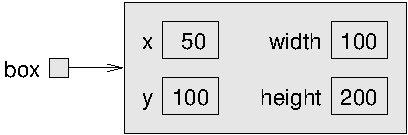
\includegraphics{figs/rectangle2.pdf}
\end{center}

\index{encapsulation}
\index{generalization}

We can encapsulate this code in a method and generalize it to move the rectangle by any amount:

\begin{code}
    public static void moveRect(Rectangle box, int dx, int dy) {
        box.x = box.x + dx;
        box.y = box.y + dy;
    }
\end{code}

The variables \java{dx} and \java{dy} indicate how far to move the rectangle in each direction.
Invoking this method has the effect of modifying the \java{Rectangle} that is passed as an argument.

\begin{code}
    Rectangle box = new Rectangle(0, 0, 100, 200);
    moveRect(box, 50, 100);
    System.out.println(box);
\end{code}

This code prints \java{java.awt.Rectangle[x=50,y=100,width=100,height=200]}.

Modifying objects by passing them as arguments to methods can be useful, but it can also make debugging more difficult because it is not always clear which method invocations do or do not modify their arguments.
%Later, I discuss some pros and cons of this programming style.

Java provides a number of methods that operate on \java{Point}s and \java{Rectangle}s.
Now would be a good time to examine the documentation for these classes.
%You can read the documentation at
%\url{http://docs.oracle.com/javase/7/docs/api/java/awt/Point.html}
%and
%\url{http://docs.oracle.com/javase/7/docs/api/java/awt/Rectangle.html}.
For example, \java{translate} has the same effect as \java{moveRect}, but instead of passing the Rectangle as an argument, you use dot notation:

\begin{code}
    box.translate(50, 100);
\end{code}

To foreshadow what's to come in future chapters, this example illustrates {\bf object-oriented programming}.
Rather than write \java{static} methods that manipulate external data (like \java{moveRect}), we make the methods non-static and bundle them with the objects themselves using dot notation.


\section{Aliasing}
\label{aliasing}

\index{reference}

Remember that when you assign an object to a variable, you are assigning a {\em reference} to an object.
It is possible to have multiple variables that refer to the same object.

\begin{code}
    Rectangle box1 = new Rectangle(0, 0, 100, 200);
    Rectangle box2 = box1;
\end{code}

This code generates a state diagram that looks like:

\begin{center}
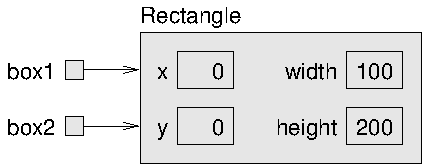
\includegraphics{figs/aliasing.pdf}
\end{center}

\index{aliasing}

The \java{box1} and \java{box2} variables refer to the same object.
In other words, this object has two names, \java{box1} and \java{box2}.
When a person in real life uses two names, it's called {\bf aliasing}.
Same thing with objects.

When two variables are aliased, any changes that affect one variable also affect the other.
For example:

\begin{code}
    System.out.println(box2.width);
    box1.grow(50, 50);
    System.out.println(box2.width);
\end{code}

The first line prints {\tt 100}, which is the width of the \java{Rectangle} referred to by \java{box2}.
The second line invokes the \java{grow} method on \java{box1}, which expands the \java{Rectangle} by 50 pixels in every direction (see the documentation for more details).
The effect is shown in the figure:

\begin{center}
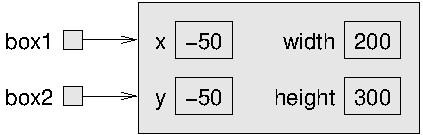
\includegraphics{figs/aliasing2.pdf}
\end{center}

Whatever changes are made to \java{box1} also apply to \java{box2}.
Thus, the value printed by the third line is {\tt 200}, the width of the expanded rectangle.
(As an aside, it is perfectly legal for the coordinates of a \java{Rectangle} to be negative.)

As you can tell even from this simple example, code that involves aliasing can get confusing fast and can be difficult to debug.
In general, aliasing should be avoided or used with care.


\section{The null keyword}

\index{null}

When you create an object variable, remember that you are storing a {\em reference} to an object.
%Until you make the variable point to an object, the value of the variable will be \java{null}.
In Java, the keyword \java{null} is a special value that means ``no object.''
You can declare and initialize object variables this way:

\begin{code}
    Point blank = null;
\end{code}

The value \java{null} is represented in state diagrams by a small box with no arrow.

\begin{center}

\includegraphics{figs/reference2.pdf}
\end{center}

\index{exception!NullPointer}
\index{run-time error}

If you try to use a \java{null} object, either by accessing an instance variable or invoking a method, Java throws a \java{NullPointerException}, prints an error message, and terminates the program.

\begin{code}
    Point blank = null;
    int x = blank.x;              // NullPointerException
    blank.translate(50, 50);      // NullPointerException
\end{code}

On the other hand, it is legal to pass a null object as an argument or receive one as a return value.
In fact, it is common to do so, for example to represent an empty set or indicate an error condition.


\section{Garbage collection}

In Section~\ref{aliasing} we talked about what happens when more than one variable refers to the same object.
What happens when {\em no} variable refers to an object?

\begin{code}
    Point blank = new Point(3, 4);
    blank = null;
\end{code}

The first line creates a new \java{Point} object and makes \java{blank} refer to it.
The second line changes \java{blank} so that instead of referring to the object, it refers to nothing (the null object).
In terms of the state diagram, we have removed the arrow between them.

\begin{center}
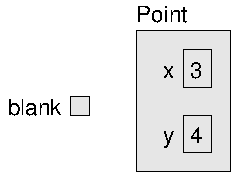
\includegraphics{figs/reference3.pdf}
\end{center}

\index{garbage collection}

If no one refers to an object, then no one can read or write any of its values, or invoke a method on it.
In effect, it ceases to exist.
We could keep the object in memory, but it would only waste space.
So periodically as your program runs, the system looks for stranded objects and reclaims them in a process called {\bf garbage collection}.
Later, the memory space occupied by the object will be available to be used as part of a new object.

You don't have to do anything to make garbage collection happen, and in general you will not be aware of it.
But you should know that it periodically runs in the background.


\section{Vocabulary}

\begin{description}

%\term{AWT}
%The Abstract Window Toolkit, one of the biggest and commonly-used Java packages.

\term{reference}
A value that indicates an object.
In a state diagram, a reference appears as an arrow.

\term{attribute}
One of the named data items (instance variables) that make up an object.
Each object (instance) has its own copy of the attributes for its class.

\term{state}
A complete description of all the variables and objects and their values, at a given point during the execution of a program.

\term{state diagram}
A snapshot of the state of a program, shown graphically.

\term{constructor}
A special method called by \java{new} to initialize an object.

\term{UML}
Unified Modeling Language, a standard way to draw diagrams for software engineering.

\term{class diagram}
An illustration of attributes and methods for a class.

\term{instance}
An example from a category.
My cat is an instance of the category ``feline things.''
Every object is an instance of some class.

\term{object-oriented programming}
A programming technique that focuses on objects rather than independent methods.

\term{aliasing}
The condition when two or more variables refer to the same object.

\term{garbage collection}
The process of finding objects that have no references and reclaiming their storage space.

\end{description}


\section{Exercises}


\begin{exercise}
For the following program:

\begin{enumerate}

\item Draw a stack diagram showing the local variables and parameters of \java{main} and \java{riddle}, and show any objects those variables refer to.

\item What is the output of this program?

\end{enumerate}

\begin{code}
    public static void main(String[] args) {
        int x = 5;
        Point blank = new Point(1, 2);

        System.out.println(riddle(x, blank));
        System.out.println(x);
        System.out.println(blank.x);
        System.out.println(blank.y);
    }

    public static int riddle(int x, Point p) {
        x = x + 7;
        return x + p.x + p.y;
    }
\end{code}

The point of this exercise is to make sure you understand the mechanism for passing objects as parameters.
\end{exercise}

\newpage

\begin{exercise}
For the following program:

\begin{enumerate}

\item Draw a stack diagram showing the state of the program just before \java{distance} returns.
Include all variables and parameters and the objects those variables refer to.

\item What is the output of this program?

\end{enumerate}

\begin{code}
    public static double distance(Point p1, Point p2) {
        int dx = p1.x - p2.x;
        int dy = p1.y - p2.y;
        return Math.sqrt(dx * dx + dy * dy);
    }

    public static Point findCenter(Rectangle box) {
        int x = box.x + box.width / 2;
        int y = box.y + box.height / 2;
        return new Point(x, y);
    }

    public static void main(String[] args) {
        Point blank = new Point(5, 8);

        Rectangle rect = new Rectangle(0, 2, 4, 4);
        Point center = findCenter(rect);

        double dist = distance(center, blank);
        System.out.println(dist);
    }
\end{code}

\end{exercise}


\begin{exercise}
The method \java{grow} is part of the \java{Rectangle} class.

\begin{enumerate}

\item What is the output of the following program?

\item Draw a state diagram that shows the state of the program just before the end of \java{main}.
Include all local variables and the objects they refer to.

\item At the end of \java{main}, are \java{p1} and \java{p2} aliased?
Why or why not?

\end{enumerate}

\begin{code}
    public static void printPoint(Point p) {
        System.out.println("(" + p.x + ", " + p.y + ")");
    }

    public static Point findCenter(Rectangle box) {
        int x = box.x + box.width / 2;
        int y = box.y + box.height / 2;
        return new Point(x, y);
    }

    public static void main(String[] args) {
        Rectangle box1 = new Rectangle(2, 4, 7, 9);
        Point p1 = findCenter(box1);
        printPoint(p1);

        box1.grow(1, 1);
        Point p2 = findCenter(box1);
        printPoint(p2);
    }
\end{code}

\end{exercise}


\begin{exercise}
\label{ex.biginteger}

You might be sick of the factorial method by now, but we're going to do one more version.

\begin{enumerate}

\item Create a new program called \java{Big.java} and write an iterative version of \java{factorial}.

\item Print a table of the integers from 0 to 30 along with their factorials.
At some point around 15, you will probably see that the answers are not right any more.
Why not?

\item \java{BigInteger} is a Java class that can represent arbitrarily big integers.
There is no upper bound except the limitations of memory size and processing speed.
Read the documentation at \url{http://docs.oracle.com/javase/7/docs/api/java/math/BigInteger.html}.

\item To use BigIntegers, you have to add \java{import java.math.BigInteger} to the beginning of your program.

\item There are several ways to create a BigInteger, but the one I recommend uses \java{valueOf}.
The following code converts an integer to a \java{BigInteger}:

\begin{code}
    int x = 17;
    BigInteger big = BigInteger.valueOf(x);
\end{code}

Type in this code and try it out.
Try printing a BigInteger.

\item Because BigIntegers are not primitive types, the usual math operators don't work.
Instead we have to use methods like \java{add}.
To add two BigIntegers, invoke \java{add} on one and pass the other as an argument.
For example:

\begin{code}
    BigInteger small = BigInteger.valueOf(17);
    BigInteger big = BigInteger.valueOf(1700000000);
    BigInteger total = small.add(big);
\end{code}

Try out some of the other methods, like \java{multiply} and \java{pow}.

\item Convert \java{factorial} so that it performs its calculation using BigIntegers and returns a BigInteger as a result.
You can leave the parameter alone---it will still be an integer.

\item Try printing the table again with your modified factorial method.
Is it correct up to 30?
How high can you make it go?
I calculated the factorial of all the numbers from 0 to 999, but my machine is pretty slow, so it took a while.
The last number, 999!, has 2565 digits.

\end{enumerate}
\end{exercise}


\begin{exercise}
Many encryption techniques depend on the ability to raise large integers to an integer power.
Here is a method that implements a (reasonably) fast technique for integer exponentiation:

\begin{code}
    public static int pow(int x, int n) {
        if (n == 0) return 1;

        // find x to the n/2 recursively
        int t = pow(x, n / 2);

        // if n is even, the result is t squared
        // if n is odd, the result is t squared times x
        if (n % 2 == 0) {
            return t*t;
        } else {
            return t*t*x;
        }
    }
\end{code}

The problem with this method is that it only works if the result is smaller than 2 billion.
Rewrite it so that the result is a \java{BigInteger}.
The parameters should still be integers, though.

You can use the BigInteger methods \java{add} and \java{multiply}, but don't use \java{pow}, which would spoil the fun.
\end{exercise}


\end{document}
